%
% DS 5110 (Blue Team) Project Proposal
%
\documentclass[12pt]{article}

%
% Packages
%
\usepackage{amsmath}
\usepackage{enumerate}
\usepackage[utf8]{inputenc}
\usepackage[toc,page]{appendix}

\RequirePackage{graphics}

\usepackage{graphicx}
\graphicspath{ {imgs/} }

%
% Document Settings
%
\setlength{\parskip}{1pc}
\setlength{\parindent}{0pt}
\setlength{\topmargin}{-3pc}
\setlength{\textheight}{9.5in}
\setlength{\oddsidemargin}{0pc}
\setlength{\evensidemargin}{0pc}
\setlength{\textwidth}{6.5in}

\title{\textbf{Flashlight}: Property Assessment Visualization for the City of Boston}
\author{Tyler Brown, Sicheng Hao, Nischal Mahaveer Chand, Sumedh Sankhe}
\date{ }


% START DOCUMENT
\begin{document}

\maketitle

\section*{Summary}

As a new home-buyer, it's easy to find out about your home
but hard to get an understanding of your neighborhood. Flashlight
makes it easier for you to see your potential neighborhood in Boston.
This discrepancy is due to current real estate websites emphasizing
individual properties rather than individual neighborhoods. Our group
communicates the differences between Boston neighborhoods using an
interactive data visualization called Flashlight.

Our dataset includes Property Assessment history from 2014-2017
\cite{Property49:online} using Boston's Open Data Hub. We enriched the 
property assessment data with coordinates from Open Addresses
\cite{OpenAddr24:online}, and neighborhood boundaries from Zillow
\cite{ZillowNe81:online}. These combined datasets provide unique
insights to new home-buyers in Boston. As open data becomes more
prevalent in cities across the United States, we can scale our insights
and models.

Our prime focus of this project is to provide information that other 
major housing websites do not, which is property assessment value and 
interior detail. Property assessment value does not relate to the 
property's selling price directly, but as the tax value. Assessment value
 has a powerful influence on home buyer's financial statements. Interior 
 detail is the information which is hard to get when viewing a property
 from outside. The interior condition of properties in Boston are widely 
distributed due to the long history of the city. Interior condition 
determines how much money and time a new owner will need to spend after 
buying the property. Since our data is a legitimate source from the 
government website \cite{Property49:online}, we are going to focus on 
how to visualize those two aspects of Boston housing. 


\section*{Methods}

We used methods for collecting, preparing, modeling, and presenting
our data. Each step of the process is detailed here.

\subsection{Data Collection}

We started with Boston's Property Assessment data from 2014-2017
\cite{Property49:online}. This dataset ``[g]ives property, or parcel,
ownership together with value information, which ensures fair assessment
of Boston taxable and non-taxable property of all types and
classifications.''\cite{Property49:online}. We wanted to use this
information because it helps us capture changes in Boston properties
over time. For example, a remodeled property would change it's property
tax assessment value we have this variable available to us.

After starting with the Property Assessment dataset, we brought in
additional datasets to increase the value of our data collection.
Neighborhoods in Boston were not named or geographically demarcated in
the Property Assessment dataset so we brought in Neighborhood Boundaries
from Zillow \cite{ZillowNe81:online} to make this distinction.
Additionally, geographic coordinates for each assessed property's address
were occasionally not coded correctly or included at all for 2017 so we 
had to bring in those values using Open Addresses
\cite{OpenAddr24:online}. Once neighborhood names, boundaries, and missing
coordinates were available, we were able to proceed to data preparation.

\subsection{Data Preparation}

There were a number of steps involved in data preparation. Transformation
of data is considered to be a part of data preparation. We detail notable
parts of our data preparation by elaborating on data audits, geocoding
missing addresses, and working with GeoJSON in Python.

\subsubsection{Data Audits}

The purpose of a data audit is to answer questions related to data
quantity and quality. We started with our Property Assessment dataset
by checking for the quantity of populated items within each variable.
About 73\% of variables were less than 70\% populated. We were able to
disregard these variables for our modeling purposes. Data quality checks
are not as easily automated but value added.

Analyzing data quality helped us understand data problems up front
such as having a non-unique primary key about $0.3\%$ of the time,
latitude and longitude were missing or corrupted about 35\% of the time,
and the ratio of unique addresses concatenated with coordinates to
unique coordinates were about $\frac{3}{1}$. We also found that the
Property Assessment data did not map to defined neighborhoods in Boston.
Understanding these shortcomings with a data audit allowed our group
to plan remediation steps early in our analysis.


\subsubsection{Geocoding Missing Addresses}

During the data audit we found about 35\% of addresses within the
Property Assessment data were not matched to any coordinate pair. Our
team work to mitigate this deficiency by leveraging the
a ``free and open global address collection'' called the
OpenAddresses \cite{OpenAddr24:online} project. There are several
strategies one can take when Geocoding (mapping address strings to
coordinate pairs) addresses. The simplest would be to use Google Maps
Geocoding API \cite{GettingS89:online}.

The Google Maps Geocoding API has a free usage tier which maxes out at
2,500 requests per day \cite{GettingS89:online}. Our data required
geocoding an order of magnitude more coordinates so this approach was
out of the question. We resolved the issue by creating 'address hashes'
for each address in the OpenAddress and Property Assessment dataset
with missing coordinates. An 'address hash' was a string concatenated
of concatenated values for street number, street name, city, and zip
code. We excluded unit number as a simplifying assumption because we
expected all unit numbers to be at the same property. Once 'address
hash' had been computed for both datasets we performed an inner join.

In some cases, this join generated a many-to-many relationship between
addresses in both datasets due to our exclusion of unit numbers. We
resolved this issue by grouping and taking the first coordinate pair.
Subsequent iterations of our analysis can be improved by adding
robustness to our geocoding procedure.

\subsubsection{Working with GeoJSON and Python}

To create the graphical interface for the map, we used Leaflet
\cite{Leafleta41:online,Leafletf18:online} - a library to show
interactive maps. The team looked at a number of ways to plot the
boundaries of each region on the map, and decided that the best way would
be to use GeoJSON \cite{RFC7946T67:online} - a format for encoding a
variety of geographic data structures. We used Zillow's shapefiles
\cite{ZillowNe81:online} to use as the base to extract region boundaries
and convert them to GeoJSON. 

Unfortunately, R did not have a robust GeoJSON library and did not 
offer the features we had in mind. We switched to Python for converting
the shapefile to GeoJSON files. We then realised that there was no way to
map the original data to the neighborhood regions which had been defined
by Zillow. To counter this, we mapped each point on the map to a region
by checking if the latitude and longitude of a point were inside a
particular region polygon. The mean interior score
of each region was used to fill the polygons, and multiple points were
clustered in higher zoom levels to reduce overplotting. Finally,
depending on the zoom level, either the regions or the points are shown.


\subsection{Data Modeling}

We used data modeling to help our user understand the differences between
neighborhoods as well as the differences between individual properties.
Two scores were generated, one as a descriptive statistic assessing the
interior of each property, and the other projected change in property
assessment value for this upcoming year. 

\subsubsection{Projected Change to Property Assessment Value}

We were able to create a representation of how property assessment
value would change in the next year. When we considered how physical
features of the property play an important role in the value of a
property, our model was more influenced more significantly by market
conditions, and surrounding neighborhoods. The Property Assessment data
did not include these market relationships. We decided to create a
simple linear model at first by using previous evaluations to predict for
the year 2017.

A more important prediction would be to predict how the price per square 
foot changes per region. We could apply the same linear model to predict 
price per sqft. First, the price per sqft was calculate for every
property parcel identification number (PID) \cite{Property49:online}. We
grouped by the region and the mean price per sqft was calculated for that
particular region by year.

Next, a linear regression model was created with 3 variables and 1 
response variable, the variables included the valuations for the year 
2014 through 2016 which predicted the evaluations for the year 2017. With 
an RMSE of \$5.45/sqft and a MAE of \$4.477/sqft the model performed 
unexcitingly. Considering all the variables were linearly related to the 
response variable. The above model was applied to predict the price per
sqft for the year 2018 taking into considerations the values from 2015
through 2017. Since there was no way to gauge the performance of this
model with real data as of now it would be interesting to see the
performance. An interesting problem would be to gauge how housing 
evaluations are done and how neighborhoods end up having such diverse 
scores even when they are next to each other.

\subsubsection{Interior Score as a Descriptive Statistic}

We combined all the columns that are related to the interior 
characteristics of properties into a single column called the interior 
score. One of the project goals was to help users understand their 
prospective properties better, not only from the neighborhood, but also
from inside. This is the kind of information which was barely accessible
for potential homebuyers. Since all interior characteristic data columns
are ordinal, we simply scaled them to 1, 2 and so on, according to what 
the group felt were high valued characteristics, with 1 being the lowest. The interior score is the sum of all such columns. Also, the score is 
exponentiated by a power of 2.5 to make the interior score normally 
distributed (approximately).


\subsection{Data Presentation}

We use Shiny Dashboard \cite{ShinyDas50:online} to present our data. The 
dashboard has two parts, a interface to filter data and the map itself. 
Filters can be used to look at specific data points on the map. The map,
rendered using Leaflet, shows the regions upon startup. Each region is
filled using the mean interior score for that region. Hovering over any
region brings up a small dialog showing statistics, like mean, max, and
min interior scores, property count, and the projected value change for
2018 in price per square feet. Zooming in hides the polygon layer and
show marker clusters and the ploygon boundaries. The clusters help with
the overplotting problem. Each cluster shows the number of properties in
the highlighted ploygon when hoving over the cluster. When a cluster is
clicked, or the map is zoomed, the clusters split to show a higher level
of detail and exposing individual property markers. When a property
marker is clicked, it brings up a popup with property details and
statistics for that property.

Filtering will help users pin down on the type of properties to view on
the map, and then the map will help users determine which neighborhood
would most suit their needs.

\section*{Results}

\subsection{Shiny App}

Our project is deployed on Shiny Server:
``https://sichenghao1992.shinyapps.io/DS5110/''


\subsection{Interesting Findings}
    \begin{enumerate}
        \item The rise in evaluations can be seen to grow very fast from 
            2014 to 2016, but the evaluations for the year 2017 have been 
            low considering the rise they have witnessed for the past 3 
            years, if the same trend follows into 2018 then the 
            evaluations will change only slightly for the year 2018.
        \item The best region in the interior score is Central. Mattapan 
          and Hyde Park have the lowest interior score. This is also the 
          intuition of Boston housing by some long-time Boston residents. 
    \end{enumerate}


\section*{Discussion}

    \begin{enumerate}
        \item One huge surprise was finding how inaccurate the 
          coordinates for properties were from government websites. Since
          we only include actual coordinates for the properties, not all 
          properties are on the interactive map.

        \item Since our model is only based on assessment values from the
          year 2014 to the year 2017, the projected values for assessment
          may be misrepresented. With more data in the future, our model 
          could perform better.
    \end{enumerate}

\section*{Statement of Contributions}

Together everyone achieves more.

\begin{itemize}
\item \textbf{Tyler Brown:} Data audit, geocoding data, preparing GeoJSON
  using Python, profiling Shiny app with Chrome DevTools, map 
  visualization in Shiny.
\item \textbf{Sicheng Hao:} Data transformation, Shiny app data filter.
\item \textbf{Nischal Mahaveer Chand:} Map visualization, finding region
  for each property in map, geocoding data to find missing latitude and
  longitude.
\item \textbf{Sumedh Sankhe:} Data cleaning and transformation, data 
  audit to apply machine learning models to predict assessment values for
  2018, linear regression for price per sqare feet for all regions, 
  initial tests to geocode data using Google's Geocoding API.
\end{itemize}


\bibliography{references} 
\bibliographystyle{ieeetr}


\section*{Appendices}

Our working repository on GitHub: 
``https://github.com/sichenghao1992/DS5110Project''


\begin{figure}
  \caption{Map Overview}
  \centering
  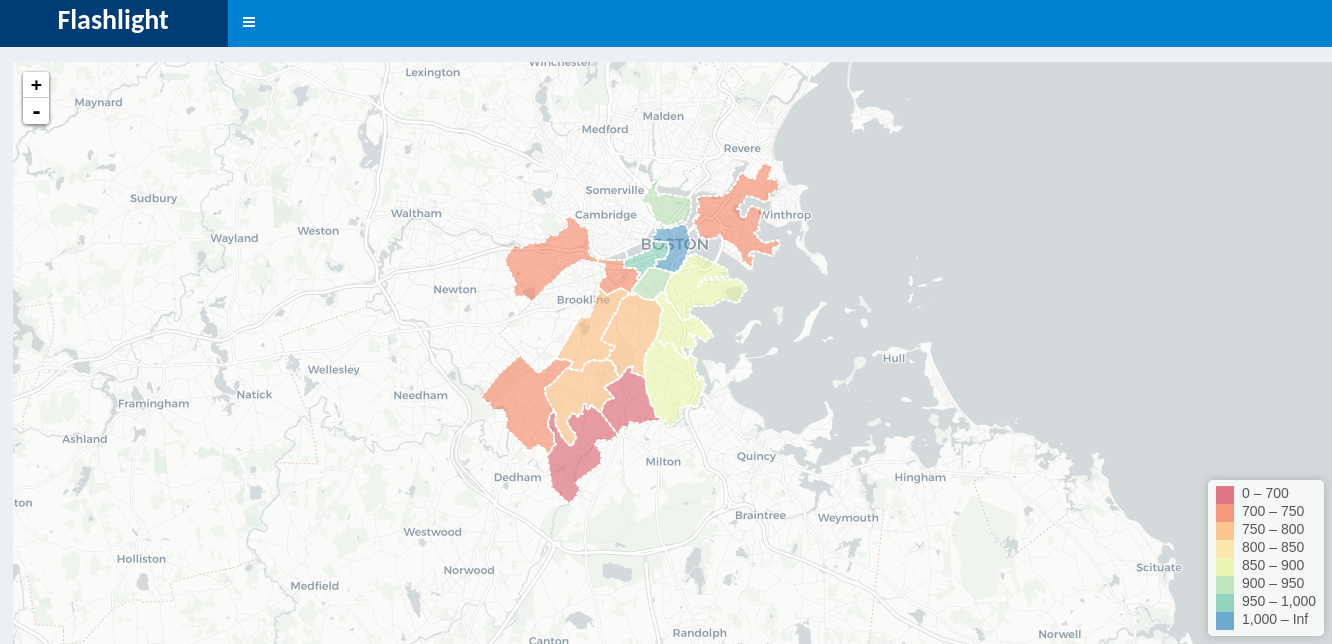
\includegraphics[width=0.85\textwidth]{map_overview}
\end{figure}

\begin{figure}
  \caption{Map Overview with Filters}
  \centering
  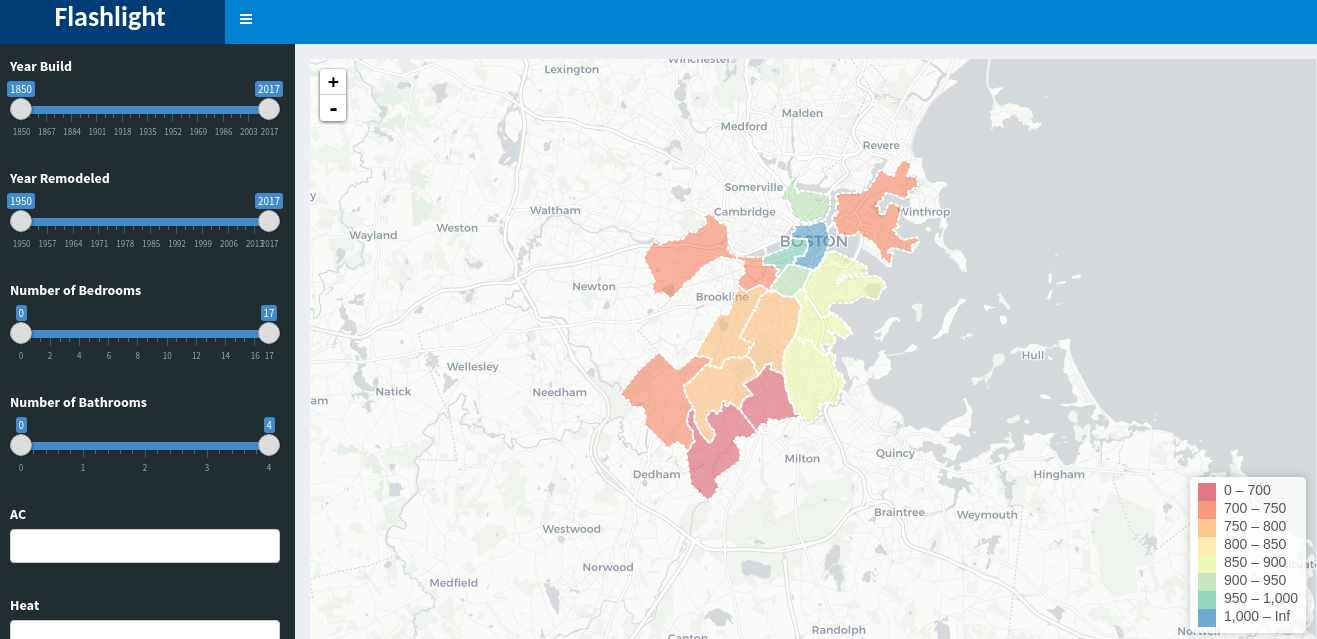
\includegraphics[width=0.85\textwidth]{map_filter_overview}
\end{figure}

\begin{figure}
  \caption{Labels for each Boston Neighborhood}
  \centering
  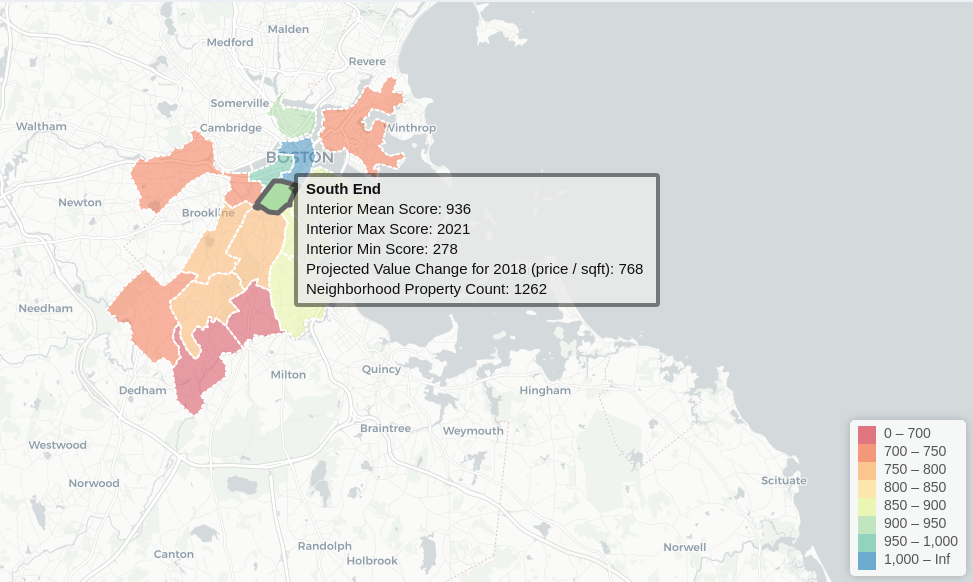
\includegraphics[width=0.85\textwidth]{region_label}
\end{figure}

\begin{figure}
  \caption{Increase Zoom to see Property Location Clusters}
  \centering
  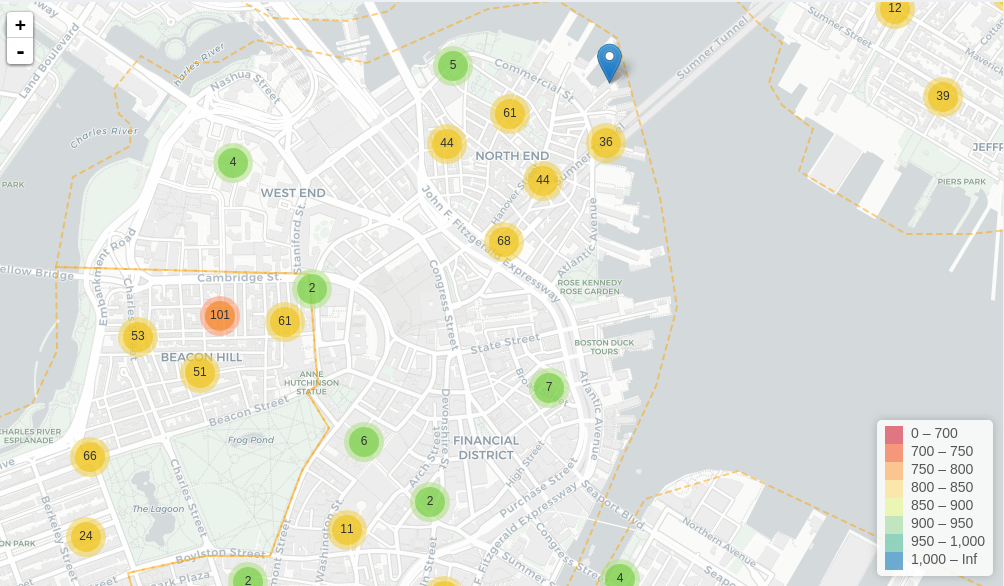
\includegraphics[width=0.85\textwidth]{showing_clusters}
\end{figure}

\begin{figure}
  \caption{Labels for each Assessed Property}
  \centering
  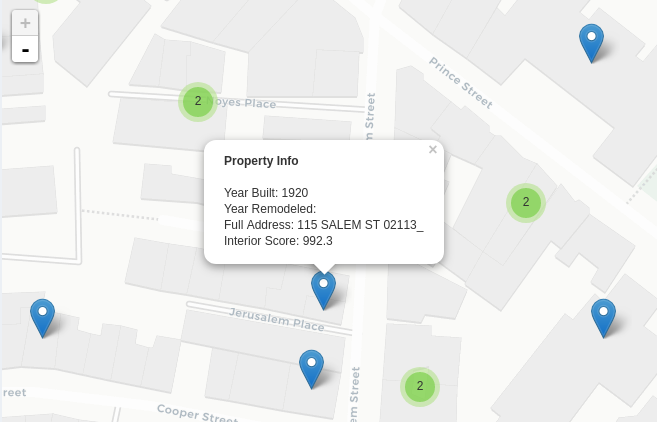
\includegraphics[width=0.85\textwidth]{individual_point_label}
\end{figure}

\begin{figure}
  \caption{Applying a Filter to Find a Properties with $>= 3$ Bathrooms}
  \centering
  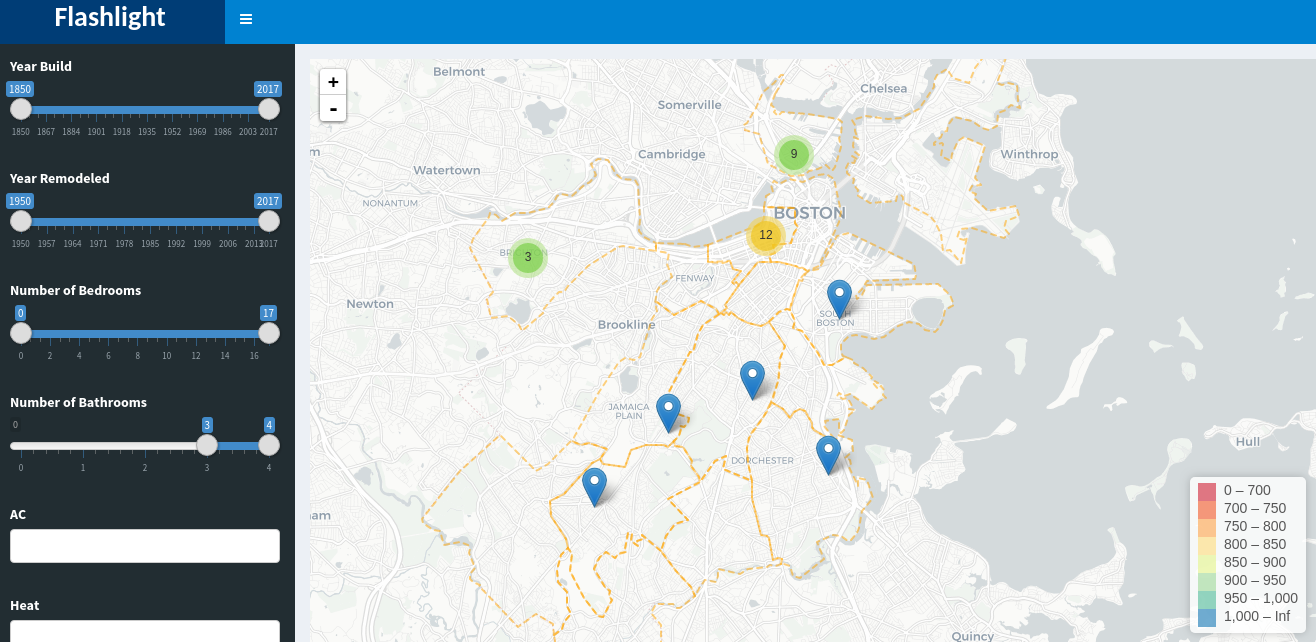
\includegraphics[width=0.85\textwidth]{bathroom_filter}
\end{figure}


\end{document}
